\documentclass[11pt,a4paper]{article}
\usepackage[utf8]{inputenc}
\usepackage[T1]{fontenc}
\usepackage[margin=2.2cm]{geometry}
\usepackage{lmodern}
\usepackage{microtype}
\usepackage{amsmath,amssymb,bm}
\usepackage[table]{xcolor}
\usepackage{booktabs}
\usepackage{tabularx}
\usepackage{float}
\usepackage{enumitem}
\usepackage[most]{tcolorbox}
\usepackage{fancyhdr}
\usepackage{needspace}
\usepackage{titlesec}
\usepackage{tikz}
\usetikzlibrary{arrows.meta,positioning,calc}
\usepackage[colorlinks=true,linkcolor=blue!60!black,urlcolor=blue!60!black]{hyperref}
\definecolor{cblue}{HTML}{2B6CB0}
\definecolor{cgreen}{HTML}{2F855A}
\definecolor{cred}{HTML}{C53030}
\definecolor{corange}{HTML}{DD6B20}
\definecolor{cgray}{HTML}{718096}
\definecolor{cpurple}{HTML}{6B46C1}
\newtcolorbox{idea}[1][]{colback=cblue!5,colframe=cblue,title={#1},fonttitle=\bfseries,breakable}
\newtcolorbox{why}[1][]{colback=cgreen!5,colframe=cgreen,title={#1},fonttitle=\bfseries,breakable}
\newtcolorbox{warn}[1][]{colback=cred!5,colframe=cred,title={#1},fonttitle=\bfseries,breakable}
\newtcolorbox{example}[1][]{colback=corange!5,colframe=corange,title={#1},fonttitle=\bfseries,breakable}
\newtcolorbox{code}[1][]{colback=cgray!7,colframe=cgray,title={#1},fonttitle=\bfseries,breakable}
\setlist{itemsep=2pt,topsep=3pt}
\pagestyle{fancy}\fancyhf{}\rhead{Part 1 of the pending run, explained}\lhead{Chapter 2 -- ball estimation}\cfoot{\thepage}
\titleformat{\section}{\Large\bfseries\color{cblue}}{\thesection}{0.6em}{}
\titleformat{\subsection}{\large\bfseries\color{cblue!80!black}}{\thesubsection}{0.6em}{}
\newcommand{\vv}{\bm v}\newcommand{\pp}{\bm p}\newcommand{\uu}{\bm u}
\newcommand{\R}{\mathbb{R}}
\begin{document}

\begin{center}
{\LARGE\bfseries Part 1 of the pending run, explained}\\[4pt]
{\large Re-running the baselines after the research audit, and the realistic-physics dataset}\\[6pt]
{\color{cgray} Written 2026-11-01 for the thesis chapter 2 (vision-based ball state estimation).\\
Every number, formula and step below matches the code at commit \texttt{df9f31a}.}
\end{center}

\tableofcontents
\newpage

%=====================================================================================================
\section{What Part 1 is, in one page}

Part 1 is the first half of \texttt{experiments/run\_overnight.sh}. It takes about \textbf{3.5 hours} and has seven steps.
Steps 1--5 redo the Phase-0 baselines with all the fixes from the research audit. Steps 6--7 check and render the new
``realistic physics'' dataset.

\begin{center}
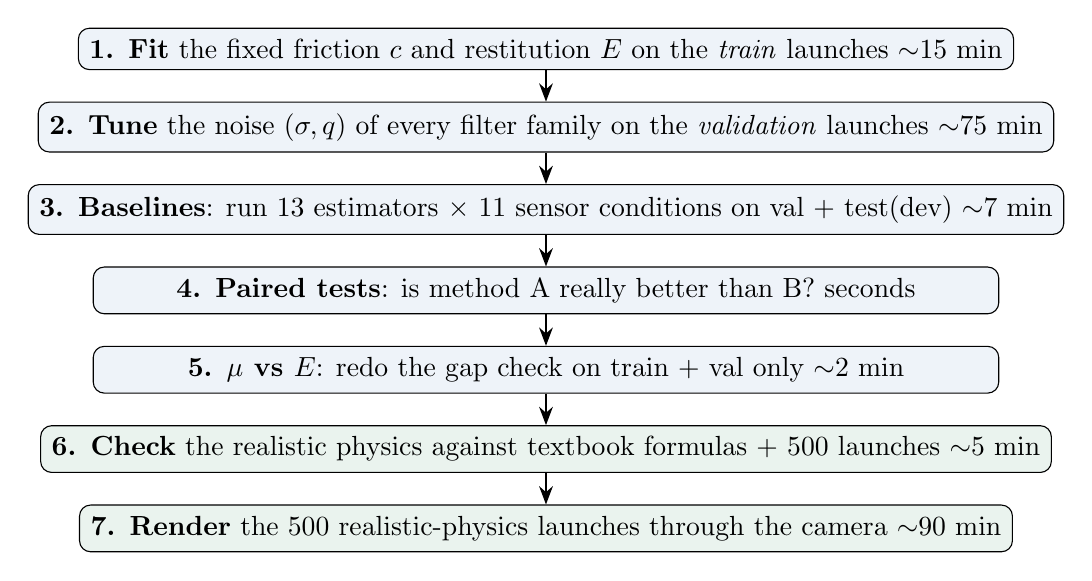
\begin{tikzpicture}[node distance=4mm, box/.style={draw,rounded corners,fill=cblue!8,minimum width=11.5cm,align=left,inner sep=4pt}]
\node[box] (a) {\textbf{1. Fit} the fixed friction $c$ and restitution $E$ on the \emph{train} launches \hfill $\sim$15 min};
\node[box,below=of a] (b) {\textbf{2. Tune} the noise $(\sigma,q)$ of every filter family on the \emph{validation} launches \hfill $\sim$75 min};
\node[box,below=of b] (c) {\textbf{3. Baselines}: run 13 estimators $\times$ 11 sensor conditions on val + test(dev) \hfill $\sim$7 min};
\node[box,below=of c] (d) {\textbf{4. Paired tests}: is method A really better than B? \hfill seconds};
\node[box,below=of d] (e) {\textbf{5. $\mu$ vs $E$}: redo the gap check on train + val only \hfill $\sim$2 min};
\node[box,below=of e,fill=cgreen!10] (f) {\textbf{6. Check} the realistic physics against textbook formulas + 500 launches \hfill $\sim$5 min};
\node[box,below=of f,fill=cgreen!10] (g) {\textbf{7. Render} the 500 realistic-physics launches through the camera \hfill $\sim$90 min};
\foreach \x/\y in {a/b,b/c,c/d,d/e,e/f,f/g} \draw[-{Stealth},thick] (\x) -- (\y);
\end{tikzpicture}
\end{center}

\begin{why}[{Why Part 1 is needed at all}]
The audit (\texttt{docs/research\_audit\_2026-11-01.md}) found problems that a reviewer would reject. Part 1 is
where the fixes become numbers:
\begin{itemize}
\item \textbf{A1}: the simulator used exactly the estimator's equations (``inverse crime''). The fix is a second dataset
  with realistic physics. Steps 6--7 create it.
\item \textbf{A2}: the test set had been looked at. From now on, results are reported on val and on a ``test (dev)'' set,
  and the true final test set is rendered only at the very end.
\item \textbf{A3}: there were no confidence intervals, and a few launches dominated. New statistics are used per launch,
  with bootstrap intervals and paired tests (Steps 3--4).
\item \textbf{B1, B2}: the measurement got two fixes: the depth correction and a new ``plane'' measurement (new conditions).
\item \textbf{B3}: the baselines were not fair. The constants are now fitted on train, and every family is tuned on its own
  (Steps 1--2).
\item \textbf{B4}: the stale-frame detector was trivially perfect. A new condition makes it fail on purpose.
\end{itemize}
\end{why}

The rest of this document explains everything you need, from the world and the camera to the filters, the metrics,
the statistics and each step, with all the maths.

%=====================================================================================================
\section{Background 1: the simulated world (``matched'' physics)}

\subsection{Arena, ball, arm}
\begin{itemize}
\item \textbf{Floor:} $2.5\times2.5$ m. The inner wall faces are at $x,y=\pm1.25$ m.
\item \textbf{Ball:} radius $r=0.03$ m. It moves only in the plane: two slide joints, no rotation, no flight.
\item \textbf{Wall limit for the centre:} $L = 1.25 - 0.03 = 1.22$ m.
\item \textbf{Arm:} a Franka Panda frozen at its home pose at the centre. The only part at ball height is the base. For the
  ball centre it is a box with centre $(c_x,c_y)=(-0.041,0)$ and half sizes $(h_x,h_y)=(0.143,0.125)$ m (the real base
  plus the ball radius).
\item \textbf{Time step} of the simulation: $\Delta t = 2$ ms.
\end{itemize}

\subsection{The physics equations (file \texttt{arena\_sim.py}, class \texttt{Arena})}
MuJoCo only integrates and renders: all contacts are switched off. The ball physics is written in Python:
\begin{enumerate}
\item \textbf{Friction} is a constant deceleration $\mu$ (m/s$^2$) against the velocity:
\[ \dot{\vv} = -\mu\,\frac{\vv}{|\vv|}. \]
If $|\vv|\le\max(10^{-3},\mu\Delta t)$, the ball is stopped exactly ($\vv=0$), because friction must never reverse the motion.
\item \textbf{Integration}: semi-implicit Euler, first $\vv \leftarrow \vv + \dot{\vv}\Delta t$, then $\pp\leftarrow \pp+\vv\Delta t$.
\item \textbf{Wall bounce}: if the centre passes $x>L$ while moving outward, then $x\leftarrow L$ and $v_x\leftarrow -E\,v_x$.
  The tangential velocity is kept. The same rule applies to $y$ and to the other walls.
\item \textbf{Arm bounce}: if the centre is inside the box, it is pushed out through the face with the smallest
  penetration, and the normal velocity becomes $-E\,v_n$ if it pointed inward.
\end{enumerate}
\textbf{Per launch}, $\mu\sim U(0.2,1.5)$ m/s$^2$ and $E\sim U(0.5,0.95)$ are drawn once and stay constant for the
whole launch.

\begin{warn}[{Important: $\mu$ is a deceleration, not a friction coefficient}]
In this project $\mu$ is in m/s$^2$. A dimensionless coefficient would be $\mu/g$. For example, $\mu=0.85$ m/s$^2$
corresponds to $0.087$. The thesis must say this clearly (audit item C1).
\end{warn}

\subsection{The 500 launches and the split}
\begin{itemize}
\item \textbf{Speeds:} $0.1,0.2,\dots,5.0$ m/s (50 values), each with 10 launches, giving 500 launches.
\item \textbf{Start and direction:} a random start position (never in or near the arm) and a random direction (seed 42).
\item \textbf{Length:} each launch is simulated for 10 s.
\item \textbf{Split} (\texttt{split\_500.json}, seed 2026): for every speed, 7 launches go to \textbf{train}, and the other 3
  go to val/test as 2+1 or 1+2, alternating. The result is 350 train, 75 val, 75 test.
\end{itemize}

\begin{idea}[{The three roles}]
\textbf{Train}: data used to \emph{learn or fit} numbers (Step 1, and later ekf-$\mu$).
\textbf{Validation (val)}: data used to \emph{choose} settings (Step 2).
\textbf{Test}: data used only to \emph{report}. If you choose anything by looking at the test results, the test is no longer
an honest estimate of performance on new data. Because our test set was looked at in Phase 0, it is now called
``test (dev)'', and the final test set will be new launches with seed 20261101 (\texttt{final\_test\_plan.json}).
\end{idea}

%=====================================================================================================
\section{Background 2: the camera and the measurement}

\subsection{Pinhole camera}
The camera looks straight down from height $H=3$ m. The image is $480\times480$ pixels with a vertical field of view of
$49^\circ$. The focal length in pixels is
\[ f = \frac{480/2}{\tan(49^\circ/2)} = \frac{240}{\tan 24.5^\circ} = 526.6\ \text{px}. \]
The image centre is $(c_u,c_v)=((480-1)/2,(480-1)/2)=(239.5,239.5)$.

A point at depth $Z$ (distance along the optical axis) and pixel $(u,v)$ lies at
\[ x = \frac{u-c_u}{f}Z,\qquad y = -\frac{v-c_v}{f}Z \]
(the minus sign is there because image rows grow downward).

\begin{example}[{Size of one pixel on the floor}]
At the ball centre's depth $Z=3-0.03=2.97$ m, one pixel is $2.97/526.6 = 5.6$ mm. The whole view is $2.73$ m wide, so
the arena plus about 5 cm of margin fits. That was the rule used to choose $49^\circ$.
\end{example}

\subsection{Detection}
The renderer gives a colour image and a depth image. The ball is green:
\begin{itemize}
\item a pixel belongs to the ball if its green value exceeds both red and blue by more than 40;
\item at least 3 such pixels are needed;
\item the \textbf{centroid} $(u,v)$ is the mean of their coordinates;
\item the depth $z_s$ is read at the pixel nearest the centroid. It is the depth of the ball's \emph{surface}, not of its centre.
\end{itemize}
If the arm hides the ball completely, there is no detection, so the frame has no measurement. If the arm hides part of
it, the centroid of the visible part is shifted. This happens even in the ``ideal'' condition and produces errors of up to
about 7 cm (audit B2).

\subsection{From surface depth to centre: the new ray correction (audit B2)}
The pixel ray through the centroid points (almost exactly) at the ball centre. Along that ray, the surface is $r$ closer
to the camera than the centre. If the ray makes an angle $\theta$ with the optical axis, then along the axis the centre is
$r\cos\theta$ deeper than the surface point:
\[ Z_c = z_s + r\cos\theta,\qquad \cos\theta = \frac{1}{\sqrt{1+a^2+b^2}},\quad a=\frac{u-c_u}{f},\ b=\frac{v-c_v}{f}. \]
The old code used $Z_c = z_s + r$, which is exact only directly below the camera ($\theta=0$). Away from the centre it puts
the ball slightly too deep, so too far out.

\begin{example}[{How big was the old error?}]
At 1.5 m from the centre, $\cos\theta = 2.97/\sqrt{2.97^2+1.5^2} = 0.893$. The depth error is
$r(1-\cos\theta)=0.03\times0.107=3.2$ mm, which gives a position error of $3.2\times1.5/2.97 = 1.6$ mm outward.
Measured on the data: the bias went from $+3.0$ mm to $+1.6$ mm at 1.3--1.8 m.

The remaining $+1.6$ mm is a pure scale of $1.0008$ (0.08\,\%). It appears even without depth (plane method), so it comes
from the pixel centroid, not from the depth. It is less than $1/3$ pixel and is documented as a residual
calibration-like error.
\end{example}

\subsection{The new ``plane'' measurement (audit B1)}
The ball centre always lies on the known plane $z=r$. So the ray can simply be intersected with that plane, with no
depth at all:
\[ x = \frac{u-c_u}{f}(H-r),\qquad y = -\frac{v-c_v}{f}(H-r). \]
Only the pixel error remains. This is what a reviewer would suggest first, so we now test it: conditions
\texttt{plane} and \texttt{all\_plane}. An optional parameter \texttt{plane\_dz} adds an error to the assumed camera
height, for calibration-error tests.

\subsection{Sensor effects (file \texttt{sensing/sensor.py})}
These are applied \emph{offline} to the stored ideal detections, so the same launch can be seen through every sensor
condition.
\begin{enumerate}
\item \textbf{Depth noise}: $z_s \leftarrow z_s + \mathcal N(0,\sigma_Z^2)$ with $\sigma_Z = k\,Z^2$. This form follows
  stereo cameras: the depth error grows with distance squared.
  \begin{itemize}
  \item $k=8.2\times10^{-4}$ gives $\sigma_Z = 8.2\times10^{-4}\times2.97^2 = 7.2$ mm (a good time-of-flight camera, ``noise'').
  \item $k=3.74\times10^{-3}$ gives $\sigma_Z=33$ mm (like an Intel D435 at 3 m, ``noise\_real'').
  \end{itemize}
  A depth error $\delta z$ moves the position by $x\,\delta z/z$. At $x=1.2$ m with 33 mm noise that is 13 mm, but at the
  image centre it is almost zero.
\item \textbf{Pixel jitter}: $u,v \leftarrow u,v+\mathcal N(0,0.3^2)$ px. On the floor that is $0.3\times5.6=1.7$ mm.
\item \textbf{Dropout}: frames are lost in bursts, following a two-state Markov chain (seen / lost); see the box below.
\item \textbf{Loss modes}:
  \begin{itemize}
  \item \emph{flagged}: the filter is told ``no measurement''.
  \item \emph{silent\_hold}: the sensor repeats the last value bit for bit and says it is valid.
  \item \emph{silent\_noisy} (new, audit B4): the sensor repeats the last detection but with \emph{fresh noise}, so it is
    not bit-identical.
  \end{itemize}
\item \textbf{Delay}: a frame captured at $t$ arrives at $t+0.04$ s. The filter knows the capture time.
\end{enumerate}

\begin{idea}[{The loss Markov chain, with its maths}]
Let $q$ be the chance per frame of going from \emph{lost} to \emph{seen}, and $p$ the chance of going from \emph{seen} to
\emph{lost}.
\begin{itemize}
\item A loss burst then lasts on average $1/q$ frames, so we choose $q=1/g$ with mean gap $g=6$ frames.
\item In the long run the fraction of lost frames is $\pi_{\text{lost}} = p/(p+q)$. We want it to equal the loss rate $r$:
\[ \frac{p}{p+q}=r \;\Rightarrow\; p = \frac{r\,q}{1-r}. \]
\item With $r=0.05$ and $g=6$: $q=0.167$ and $p=0.00877$. Check: $p/(p+q)=0.05$.
\end{itemize}
The loss chain has its own random generator, so every condition with the same loss parameters loses
\emph{the same frames}. That makes conditions directly comparable (``paired'').
\end{idea}

\subsection{The 11 sensor conditions}
\begin{center}\small
\begin{tabularx}{\linewidth}{@{}l>{\raggedright\arraybackslash}X>{\raggedright\arraybackslash}X@{}}\toprule
Name & What it adds & Question it answers\\\midrule
ideal & nothing (but see B2: centroid bias, occlusions) & best case\\
noise & $\sigma_Z=7$ mm, jitter 0.3 px & good depth camera\\
dropout\_flagged & 5\,\% loss, bursts of 6, flagged & missing frames\\
dropout\_silent & same losses, repeated bit-identical & frozen camera\\
delay & 40 ms latency & latency\\
all & noise + flagged dropout + delay & everything (optimistic)\\
noise\_real & $\sigma_Z=33$ mm, jitter 0.3 px & D435-like depth\\
all\_real & noise\_real + flagged dropout + delay & everything (realistic)\\\midrule
\textbf{plane} (new) & as noise\_real, but $(x,y)$ from the plane, no depth & B1: is depth needed?\\
\textbf{all\_plane} (new) & as all\_real, but plane measurement & B1 in the hard case\\
\textbf{dropout\_silent\_noisy} (new) & noise + losses repeated with fresh noise & B4: stale frames that cannot be detected\\\bottomrule
\end{tabularx}\end{center}

\begin{idea}[{Pairing inside the plane conditions}]
In ``plane'' mode the code still draws the depth-noise random number and throws it away. So \texttt{plane} receives
exactly the same pixel-jitter values as \texttt{noise\_real} with the same seed. The two conditions then differ
\emph{only} in how $(x,y)$ is computed, and a paired comparison measures exactly that.
\end{idea}

%=====================================================================================================
\section{Background 3: the estimators}

All estimators share one interface: \texttt{update(t, xy, valid)} at every frame, and \texttt{forecast(dt)}, which
predicts the state \texttt{dt} seconds after the filter's own time.

\subsection{fd: finite differences}
The position is the latest measurement. The velocity is the difference of the last two valid measurements divided by
their time difference. The forecast is a straight line: $\pp(t+\Delta)=\pp+\vv\Delta$. There is no friction and there are
no walls. It is the simplest possible baseline.

\subsection{The motion model of the EKFs (\texttt{estimators/model.py})}
This is the same physics as the matched simulator, applied in sub-steps $h\le5$ ms during filtering and $h\le10$ ms
when forecasting:
\begin{enumerate}
\item friction: if $c\,h\ge|\vv|$ the ball stops, else $\vv\leftarrow\vv - c\,h\,\vv/|\vv|$;
\item move: $\pp\leftarrow\pp+\vv h$;
\item walls: if $x>L$ then $x\leftarrow L-E(x-L)$ and $v_x\leftarrow -E v_x$. The overshoot is mirrored and shortened by $E$:
  this is the exact position if the bounce happened inside the step;
\item arm box: a \emph{swept} test on the segment from the old to the new position finds which face was crossed first,
  and then mirrors in the same way. Because the whole segment is tested, a long step can neither pick the wrong face nor
  jump over a corner.
\end{enumerate}

\subsection{The Extended Kalman Filter (EKF19, after Liu et al.\ 2021)}
\textbf{State} $\bm s=(x,y,v_x,v_y)$. \textbf{Uncertainty}: the covariance matrix $P$ ($4\times4$): the diagonal holds the
variances, the off-diagonal entries the links between the numbers.

\paragraph{Start.} At the first valid measurement $\bm z$: $\bm s=(z_x,z_y,0,0)$ and
$P_0=\mathrm{diag}(\sigma^2,\sigma^2,\sigma_{v0}^2,\sigma_{v0}^2)$ with $\sigma_{v0}=3$ m/s. The first frame says nothing
about the velocity, hence the large value.

\paragraph{Predict} (in sub-steps $h$ up to the next measurement time):
\[ \bm s \leftarrow g(\bm s),\qquad P \leftarrow F P F^\top + Q. \]
Here $g$ is the motion model above and $F=\partial g/\partial\bm s$ is its Jacobian, the ``derivative matrix''. For
friction:
\[ \frac{\partial \vv'}{\partial \vv} = I - \frac{c h}{|\vv|}\left(I - \hat{\vv}\hat{\vv}^\top\right),\qquad
\frac{\partial \pp'}{\partial \vv} = h\,I. \]
This means friction shrinks uncertainty \emph{across} the motion direction a little, but not \emph{along} it (because
$\hat\vv\hat\vv^\top$ removes the along-component).

\begin{warn}[{A known approximation of this baseline (audit B5)}]
EKF19 does \emph{not} put the bounce into $F$: after a bounce the mean is mirrored but $P$ is not. ekf-$\mu$ (Part 2)
does it correctly. For the baseline we keep Liu et al.'s version on purpose and label it as such.
\end{warn}

\paragraph{The process noise $Q$, derived.}
$Q$ says how much the true motion can differ from the model in one sub-step. The standard choice is ``white-noise
acceleration'': the ball receives random accelerations $a(t)$ with spectral density $q$ (units m$^2$/s$^3$). Over a step
$h$ they change the velocity by $\delta v=\int_0^h a\,dt$ and the position by $\delta p=\int_0^h (h-t)a\,dt$. With
$\mathbb E[a(t)a(t')]=q\,\delta(t-t')$:
\[ \mathbb E[\delta v^2]=q h,\qquad \mathbb E[\delta p\,\delta v]=q\frac{h^2}{2},\qquad \mathbb E[\delta p^2]=q\frac{h^3}{3}. \]
So per axis $Q=q\begin{pmatrix}h^3/3 & h^2/2\\ h^2/2 & h\end{pmatrix}$. This is exactly what the code builds.
A large $q$ means ``I trust my motion model little''.

\paragraph{Correct (update)} with measurement $\bm z$ of the position, $H=[I_2\ 0]$:
\begin{align*}
\bm y &= \bm z - H\bm s &&\text{innovation: measured minus predicted}\\
S &= H P H^\top + R,\quad R=\sigma^2 I_2 &&\text{how big $\bm y$ is expected to be}\\
K &= P H^\top S^{-1} &&\text{Kalman gain}\\
\bm s &\leftarrow \bm s + K\bm y,\qquad P\leftarrow (I-KH)P.
\end{align*}

\begin{example}[{The gain in one dimension}]
Suppose the predicted position is unsure by 10 mm and the camera by 5 mm. Then
$K = 10^2/(10^2+5^2) = 0.8$: the filter moves 80\,\% of the way to the measurement. With a 1 mm camera,
$K=100/101\approx0.99$. With a 30 mm camera, $K=100/1000=0.1$.
\end{example}

\paragraph{Gate and policies.}
$d^2=\bm y^\top S^{-1}\bm y$ measures how surprising a measurement is. If the filter is right, $d^2$ follows a
$\chi^2$ distribution with 2 degrees of freedom, and $d^2>9.21$ happens in only 1\,\% of frames ($\chi^2_{2}$, 99\,\%).
\begin{itemize}
\item \texttt{none}: never reject.
\item \texttt{hybrid}: reject a surprising measurement; after 3 rejections in a row, reset to the measurement with $P=I$.
\end{itemize}

\subsection{The variants}
\begin{itemize}
\item \textbf{cvkf}: the same EKF with $c=0$ and no walls or arm: a constant-velocity Kalman filter.
\item \textbf{ekf19}: friction $c=0.85$, $E=0.725$ (the midpoints of the sampling ranges).
\item \textbf{ekf19b}: ekf19 plus extra uncertainty at a bounce. If a velocity component changes sign, add
  $(\sigma_E|v|)^2$ to its variance with $\sigma_E=0.13$, the standard deviation of $U(0.5,0.95)$:
  $0.45/\sqrt{12}=0.13$.
\item \textbf{ekf19b\_fit} (new, audit B3): ekf19b with $c,E$ fitted on train (Step 1).
\item \textbf{oracle}: ekf19 or ekf19b with the \emph{true} $\mu,E$ of each launch. This is the upper bound for any
  constant-parameter filter.
\item \textbf{+stale (StaleGuard)}: a wrapper. A valid measurement bit-identical to the previous one is treated as
  missing. A real noisy sensor never repeats exactly, but a frozen one does.
\end{itemize}

\begin{center}\small
\begin{tabularx}{\linewidth}{@{}>{\raggedright\arraybackslash}X>{\raggedright\arraybackslash}X>{\raggedright\arraybackslash}X@{}}\toprule
\multicolumn{3}{@{}l}{\textbf{The 13 estimators of Step 3}}\\\midrule
fd, fd+stale & cvkf & ekf19-none, ekf19-hybrid\\
ekf19b-none, ekf19b-none+stale, ekf19b-hybrid & ekf19b\_fit-none+stale & ekf19\_oracle-none, ekf19\_oracle-hybrid\\
ekf19b\_oracle-none, ekf19b\_oracle-none+stale & & \\\bottomrule
\end{tabularx}\end{center}

%=====================================================================================================
\section{Background 4: how errors are measured}

\subsection{When and what (file \texttt{estimators/metrics.py})}
The filter is scored at the \textbf{arrival} time $t_a=t_{\text{capture}}+\text{delay}$, the moment the robot would
actually have the information. At that moment:
\begin{itemize}
\item \textbf{now\_pos}: position error at $t_a$ (the filter forecasts from its own time to $t_a$);
\item \textbf{now\_vel}: velocity error at $t_a$ (m/s);
\item \textbf{h0.2, h0.5, h1.0}: position error of the forecast $0.2$, $0.5$, $1.0$ s after $t_a$, compared with the true
  position then. h0.5 is the main number, because a robot catch needs a forecast of roughly that horizon.
\end{itemize}
\textbf{Which frames are scored}: every 6th frame (10 per second), only after 0.1 s of warm-up, only while the true ball
speed is at least 0.05 m/s (no score for a ball at rest), and a forecast only if its target time is still inside the 10 s
recording. The truth is the 500 Hz simulator trajectory, interpolated linearly.

\subsection{Statistics (file \texttt{estimators/stats.py}): why per launch}
\begin{example}[{Why pooling frames is misleading}]
A launch at 5 m/s can be scored on about 90 frames, one at 0.1 m/s on only 1--3 frames. Pooling all frames into one
RMS lets the fast launches decide the result: 69\,\% of all scored frames come from launches at $\ge2.5$ m/s. Also,
the frames of one launch are strongly linked (the same ball, the same $\mu$). So they are not 90 independent pieces of
evidence, but closer to one.
\end{example}

\paragraph{Per-launch RMS.} For launch $i$ with scored errors $e_{i1},\dots,e_{in_i}$:
\[ \mathrm{RMS}_i = \sqrt{\tfrac{1}{n_i}\textstyle\sum_k e_{ik}^2}. \]
Every launch then counts once. The tables show the \textbf{launch mean} $\bar R=\frac1N\sum_i \mathrm{RMS}_i$, the
\textbf{launch median}, and, for continuity with Phase 0, the old pooled RMS.

\paragraph{Bootstrap 95\,\% interval.} How sure are we about $\bar R$, given only $N=75$ launches?
\begin{enumerate}
\item Draw $N$ launches \emph{with replacement} from the $N$ we have (some twice, some not at all).
\item Compute $\bar R$ for this new set.
\item Repeat 2000 times. The 2.5\,\% and 97.5\,\% points of the 2000 values form the interval.
\end{enumerate}
The idea: our 75 launches are a sample of all possible launches, and resampling them imitates drawing new samples.
A wide interval means ``we cannot tell precisely''.

\subsection{Paired comparison of two methods}
Two methods A and B run on the \emph{same} launches with the \emph{same} noise. For each launch take the difference
$d_i=\mathrm{RMS}_i^{A}-\mathrm{RMS}_i^{B}$ (negative means A is better). Pairing removes the large launch-to-launch
spread (fast vs slow, many vs few bounces), so small but real differences become visible.
\begin{itemize}
\item \textbf{Mean difference} with a bootstrap 95\,\% interval. If the interval does not contain 0, the difference is real.
\item \textbf{Wilcoxon signed-rank test}: rank the $|d_i|$ from small to large, then add up the ranks of the positive
  differences. If A and B were equally good, positive and negative differences would be equally likely, and that sum
  would be near half of the total. The p-value is the chance of a sum at least this extreme under ``equally good''. A small
  p (e.g.\ $<0.01$) means the difference is very unlikely to be luck. The test uses ranks, not values, so a single crazy
  launch cannot dominate it.
\item \textbf{Win rate}: the fraction of launches where A is better.
\end{itemize}

\begin{example}[{Wilcoxon on 5 launches}]
Take $d=(-12,-3,+1,-8,-20)$ mm. The ranks of $|d|$ are $(4,2,1,3,5)$. The only positive difference is $+1$, with rank 1,
so the statistic is $W^+=1$. Under ``equally good'' each sign is a coin flip, so there are $2^5=32$ sign patterns.
Exactly 2 of them have $W^+\le1$ (no positive differences, or only the smallest one positive). So the one-sided chance
is $2/32$ and the two-sided p-value is $4/32=0.125$. Five launches are too few to be sure, which is why we need 75.
\end{example}

\begin{warn}[{Many comparisons}]
Step 4 makes dozens of comparisons. At $p<0.05$, about 1 in 20 ``significant'' results would appear by chance even if
nothing differed. For the thesis we interpret only the comparisons planned in advance (listed in Step 4), report the
intervals and not only p-values, and use a strict level (e.g.\ $p<0.01$).
\end{warn}

%=====================================================================================================
\section{Step 1 -- fit $c$ and $E$ on train}
\noindent\textbf{Script:} \texttt{step\_0k\_fit\_constants\_train.py}\par\medskip
\begin{why}[{Purpose (audit B3)}]
ekf19b used $c=0.85$ and $E=0.725$, the midpoints of the ranges the launches were \emph{drawn} from. That is knowledge
of the data generator, which a real system does not have. Phase 1's learned filters fit their numbers on the train
launches, so the fair fixed-constant baseline must be fitted on the same launches, with the same criterion.
\end{why}
\textbf{Procedure.}
\begin{enumerate}
\item For every pair $(c,E)$ on the grid
  \[ c\in\{0.45,0.55,\dots,1.05\}\ (7\text{ values})\ \times\ E\in\{0.625,0.675,\dots,0.825\}\ (5\text{ values}), \]
  run ekf19b-none+stale on all 350 train launches.
\item The noise $(\sigma,q)$ comes from the Phase-0 validation tuning of that condition.
\item Score each pair by the launch-mean h0.5 RMS. The pair with the lowest score wins.
\item This is done in condition \textbf{ideal}, because physical constants do not depend on the camera. It is repeated in
  \textbf{all\_real} only as a check: if the best $(c,E)$ is similar, the fit is robust.
\end{enumerate}
\textbf{Why can the best $c$ differ from 0.85?} The forecast error is not symmetric in $c$. A filter with too high $c$
predicts that the ball stops early, and the error then grows with the remaining travel. Balls with high $\mu$ stop sooner
and are scored on fewer frames, but per-launch RMS weights every launch equally. So the best constant may well be below
or above the mean $\mu$. Finding out is the point of the step.

\textbf{Then, a single coordinate-descent pass}: $(c,E)$ is fitted with fixed $(\sigma,q)$, and Step 2 re-tunes
$(\sigma,q)$ with the fitted $(c,E)$. (A full joint fit would iterate. One pass is standard and is stated as such.)

\textbf{Output}: \texttt{outputs/fit\_constants\_train.json} (best $c,E$, the full grid, an ``on grid edge'' flag),
log \texttt{fit\_constants\_train.log}.

\textbf{What to look at}: the printed grid (lowest value marked \texttt{*}); whether the best value lies on the grid edge
(then the grid must be widened); and how much better it is than $(0.85,0.725)$.

%=====================================================================================================
\section{Step 2 -- tune the noise on validation}
\noindent\textbf{Script:} \texttt{step\_0i\_tune\_ekf\_noise.py}\par\medskip
\begin{why}[{Purpose}]
$\sigma$ (how much the filter trusts the camera) and $q$ (how much it trusts its motion model) change the results a lot,
and the best values depend on the sensor condition. Tuning them on \emph{validation} launches keeps train and test clean.
New in this version:
\begin{itemize}
\item every family is tuned on its own, so every method gets the same tuning effort;
\item the criterion is the launch mean, not pooled frames;
\item the new conditions are included.
\end{itemize}
\end{why}
\begin{center}\small
\begin{tabular}{@{}llll@{}}\toprule
Family & Tuned with & Grid $\sigma$ (mm) & Grid $q$ (m$^2$/s$^3$)\\\midrule
ekf & ekf19b-none+stale ($c,E$ midpoints) & 2, 3, 5, 8, 12, 20, 30 & 0.03, 0.1, 0.5, 2, 5, 20\\
ekf\_fit & ekf19b\_fit-none+stale ($c,E$ from Step 1) & same & same\\
oracle & ekf19b\_oracle-none+stale (true $\mu,E$) & same & same\\
cvkf & cvkf & 1, 2, 3, 5, 8, 12 & 2, 5, 20, 50, 200, 1000\\\bottomrule
\end{tabular}\end{center}
\begin{itemize}
\item \textbf{Total work}: 162 settings $\times$ 75 val launches $\times$ 11 conditions $\approx$ 134\,000 filter runs.
\item \textbf{Criterion}: launch-mean h0.5 RMS on val. The lowest wins, separately for every family and condition.
\item \textbf{Why cvkf has its own, wider grid}: it has no friction or walls, so it needs a very large $q$ to follow the
  slowing and the bounces. In Phase 0 its best $q$ was on the grid edge in 5 of 8 conditions.
\item \textbf{Why the oracle is tuned too}: an upper bound should be the \emph{best} that the true constants allow.
  Phase 0 gave it ekf19b's settings.
\end{itemize}
\textbf{Output}: \texttt{outputs/ekf\_tuning\_val.json} (per family and condition: the best $\sigma$, $q$, the score, an
edge flag), log \texttt{ekf\_tuning\_val.log} (all grids printed). The Phase-0 version is kept as
\texttt{ekf\_tuning\_val\_v2\_phase0.json}.

\begin{warn}[{A point to watch (seen in a smoke test)}]
Tuning on forecast error tends to choose a $\sigma$ (e.g.\ 5 mm) much larger than the real camera noise (about 1 mm in
``ideal''). The filter then forecasts well but is badly ``over-cautious'': its claimed uncertainty is much larger than its
real errors. We will measure this with the NIS/NEES consistency test in Part 2. It is a research finding, not a bug.
\end{warn}

%=====================================================================================================
\section{Step 3 -- the baselines}
\noindent\textbf{Script:} \texttt{step\_0d\_baselines\_with\_arm.py}\par\medskip
\textbf{Procedure}: the 13 estimators run on the 75 val + 75 test(dev) launches, in all 11 conditions. Each uses its
family's tuned noise, and ekf19b\_fit also uses the Step-1 constants. The noise seed of launch $i$ is $1000+i$
everywhere, so every estimator sees exactly the same noisy measurements.

\textbf{Printed tables} (for TEST (dev) and VAL, every condition): for now\_pos, now\_vel, h0.5 and h1.0, each cell shows
\[ \text{launch mean}\ [\text{95\,\% interval}]\quad \text{launch median}\quad \text{pooled RMS}. \]

\textbf{Outputs}:
\begin{itemize}
\item \texttt{outputs/baselines\_v3\_val\_test.json}: the summaries;
\item \texttt{outputs/baselines\_v3\_errors.pkl.gz}: \emph{every} per-frame error of every estimator, launch and
  condition. Any new statistic can then be computed later without re-running;
\item the log \texttt{baselines\_v3\_val\_test.log}.
\end{itemize}

\textbf{Why only val and test(dev), not all 500?} The ``ALL 500'' numbers of Phase 0 mixed in the train launches, on which
Step 1 now fits. Reporting on data that was used for fitting would flatter the fitted method.

%=====================================================================================================
\section{Step 4 -- paired tests}
\noindent\textbf{Script:} \texttt{step\_0j\_paired\_tests.py}\par\medskip
This step uses the saved errors from Step 3; it runs nothing new. For TEST (dev) and VAL, and for h0.5 and now\_pos, it
reports the mean difference with its interval, the Wilcoxon p-value and the win rate.
\begin{center}\small
\begin{tabular}{@{}p{6.3cm}p{8.3cm}@{}}\toprule
Comparison (every condition) & Question\\\midrule
ekf19b\_fit vs ekf19b & Do train-fitted constants beat the generator midpoints?\\
oracle vs ekf19b & How big is the gap that Phase 1 tries to close?\\
ekf19b-hybrid vs ekf19b+stale & Does the gate help or hurt?\\
ekf19b+stale vs cvkf & How much does the physics model add?\\\midrule
\multicolumn{2}{@{}l}{Across conditions (ekf19b+stale and oracle):}\\
plane vs noise\_real & B1: is the plane measurement better than D435-like depth?\\
all\_plane vs all\_real & B1 in the realistic full condition\\
noise vs ideal; noise\_real vs noise & What does each level of camera noise cost?\\
dropout\_silent\_noisy vs noise & B4: what do undetectable stale frames cost?\\\bottomrule
\end{tabular}\end{center}
\textbf{Output}: \texttt{outputs/paired\_tests\_v3.json} and \texttt{.log}.

%=====================================================================================================
\section{Step 5 -- $\mu$ vs $E$ on train + val}
\noindent\textbf{Script:} \texttt{step\_1a\_mu\_vs\_e\_gap.py}\par\medskip
\begin{why}[{Purpose (audit A2)}]
The decision ``put $\mu$ into the state first, $E$ later'' was taken from a check on all 500 launches, \emph{including} the
test launches. It is redone on train + val only (425 launches), with launch-level statistics. If the conclusion holds,
the decision is clean. If it changes, we must reconsider Phase 1.
\end{why}
Four filters (ekf19b-none+stale, ekf-family noise), in ideal and all\_real:
\begin{center}\small
\begin{tabular}{@{}lcc@{}}\toprule
Variant & friction $c$ & restitution $E$\\\midrule
nominal & 0.85 & 0.725\\
true $\mu$ only & true & 0.725\\
true $E$ only & 0.85 & true\\
true both (= oracle) & true & true\\\bottomrule
\end{tabular}\end{center}
For h0.5 and h1.0 it reports the launch mean [interval], the median, and the paired difference against nominal.
Earlier result (all 500, pooled): knowing $\mu$ took the typical error from 47 to 6 mm, knowing $E$ only from 47 to 43 mm.
\textbf{Output}: \texttt{outputs/mu\_vs\_e\_gap\_trainval.json} and \texttt{.log}.

%=====================================================================================================
\section{Step 6 -- check the realistic physics}
\noindent\textbf{Script:} \texttt{step\_0l\_check\_mismatch\_physics.py}\par\medskip

\subsection{Why a second physics at all (audit A1)}
If the simulator uses exactly the estimator's equations, a method that estimates those equations' constants looks
almost perfect. The oracle's typical 0.5 s error is only about 10 mm. Real balls behave differently. The ``mismatch''
simulator (\texttt{MismatchArena} in \texttt{arena\_sim.py}) adds well-known effects that \emph{no} estimator contains.
A conclusion only counts if it holds on both datasets.

\subsection{The realistic physics, with the maths}
The ball now has a spin $\bm\omega$ (3 numbers), tracked in Python. Rendering is unchanged: a uniform green sphere looks
the same when it spins. The ball is a solid sphere with moment of inertia $I=\frac25 m r^2$.

\paragraph{(a) Sliding and rolling.} The floor touches the ball at the point $-r\hat z$ below the centre. That point moves
with the \emph{slip velocity}
\[ \uu = \vv + \bm\omega\times(-r\hat z) = (v_x - r\omega_y,\; v_y + r\omega_x). \]
\begin{itemize}
\item $\uu=0$ means \emph{rolling} (no sliding at the contact).
\item While $\uu\ne0$ the ball \emph{slides}, and floor friction $\mu_s g$ acts against $\uu$:
\[ \dot\vv = -\mu_s g\,\hat\uu,\qquad \dot{\bm\omega} = \frac{\bm r_c\times\bm F}{I} = \frac{5\mu_s g}{2r}\,(\hat z\times\hat\uu). \]
\item Putting both into $\dot\uu=\dot\vv - r\,\dot{\bm\omega}\times\hat z$, and using $(\hat z\times\hat\uu)\times\hat z=\hat\uu$:
\[ \dot\uu = -\mu_s g\,\hat\uu - \tfrac52\mu_s g\,\hat\uu = -\tfrac72\,\mu_s g\,\hat\uu. \]
\item So the slip shrinks at the constant rate $\frac72\mu_s g$, and rolling starts after $t_r = \dfrac{2|\uu_0|}{7\mu_s g}$.
\item For a ball launched without spin, $\uu_0=\vv_0$, so at that moment
  $|\vv| = v_0 - \mu_s g\,t_r = v_0 - \tfrac27 v_0 = \tfrac57 v_0$.
\end{itemize}
The same result follows from angular momentum about the contact point, which friction cannot change (it acts at that
point):
\[ m r v_0 = m r v_f + I\frac{v_f}{r}\;\Rightarrow\; v_f = \frac{v_0}{1+2/5}=\frac57 v_0. \]
\textbf{The estimator does not know this.} It assumes one constant deceleration, while the truth decelerates strongly
($\mu_s g\approx 1.5$--4 m/s$^2$) for a short time and then weakly.

\paragraph{(b) Rolling resistance.} While rolling, the deceleration is $a_{\text{roll}} = a_0(1+k|\vv|)$, against $\vv$, and
the spin follows the rolling condition. Literature values for carpet are rolling-resistance coefficients of about
0.013--0.047, i.e.\ $a_0\approx0.1$--0.5 m/s$^2$; your choice was the range 0.1--0.8 m/s$^2$.

\paragraph{(c) Launch spin.} The launch slip is $\uu_0 = s\,\vv_0$ with $s\sim U(0,1)$. $s=0$ means already rolling (e.g.\
released from a ramp); $s=1$ means pure sliding (struck).

\paragraph{(d) Floor tilt.} A tilt $\alpha$ in direction $\phi$ adds $\bm g_t = g\sin\alpha\,(\cos\phi,\sin\phi)$. For a
\emph{rolling} sphere only $\frac57$ of it accelerates the centre:
\[ m a = m g_t - F,\quad I\frac{a}{r}=F r\;\Rightarrow\; a\left(1+\frac{I}{mr^2}\right)=g_t \;\Rightarrow\; a=\frac{g_t}{1.4}=\frac57 g_t. \]
The ball stays at rest if $\frac57 g_t < a_0$. With $\alpha\le0.15^\circ$, $\frac57 g\sin\alpha\le0.018<0.1$, so a resting
ball never starts rolling by itself.

\paragraph{(e) Impacts with walls and the arm.} The impact normal $\bm n$ points into the arena (or out of the arm box).
\begin{itemize}
\item \textbf{Normal}: $v_n' = -e(v_n)\,v_n$ with a restitution that falls with impact speed,
  $e = \mathrm{clip}(e_0-\beta|v_n|,\;0.3,\;0.98)$. There is a separate $e_0$ for the walls ($U(0.55,0.95)$) and the
  arm ($U(0.40,0.90)$).
\item \textbf{Normal impulse} per unit mass: $J_n=(1+e)|v_n|$.
\item \textbf{Friction at the contact}: the contact is at the ball's centre height. Its slip in the wall plane has a
  horizontal part (along the wall) and a vertical part (from the rolling spin). A Coulomb impulse opposes it, of size
  $\min(\mu_w J_n,\ \text{the impulse that stops the slip})$, with $\mu_w\sim U(0.1,0.3)$ (Mathavan et al.\ 2010
  measured 0.14). The horizontal part changes the tangential speed; the vertical part only changes the spin, because the
  floor holds the ball down.
\item \textbf{Exact timing}: the ball is moved back to the impact point (time $\tau=\text{overshoot}/|v_n|$ before the end
  of the step), its velocity is changed, and it is moved forward again with the new velocity. Positions are mirrored,
  not clamped (fixing audit C4 for this dataset).
\end{itemize}

\begin{example}[{The biggest difference: a rolling ball hits a wall head-on}]
Before the impact the ball rolls with speed $v$ and spin $\omega=v/r$ (topspin).
\begin{itemize}
\item After the impact the velocity is $-e v$, but the spin still turns ``forward''. The ball now slides, and the slip
  slows its return.
\item Wall friction first removes a fraction $f=\frac52\mu_w(1+e)$ of the spin (if the slip is not stopped completely).
\item By conservation of angular momentum about the floor contact, the ball finally rolls back at
\[ v_{\text{final}} = \frac{-e v + \frac25(1-f)v}{1+\frac25} = -\frac{5e-2(1-f)}{7}\,v. \]
\item With $e=0.8$: $f=0$ gives $0.29\,v$, and $\mu_w=0.14$ ($f=0.63$) gives $0.47\,v$.
\end{itemize}
The estimators assume $0.8\,v$. This is a large, realistic model error, and it is exactly the kind of thing the
mismatch dataset is meant to expose.
\end{example}

\paragraph{Parameter ranges} (per launch, uniform; your decisions of 2026-11-01): $\mu_s$ 0.15--0.40; $a_0$ 0.10--0.80
m/s$^2$; $k$ 0--0.1 s/m; $s$ 0--1; $e_0$ walls 0.55--0.95, arm 0.40--0.90; $\beta$ 0--0.04 s/m; $\mu_w$ 0.10--0.30;
tilt 0--0.15$^\circ$ in a random direction.

\paragraph{Pairing.} The mismatch launches keep \emph{the same start position and velocity} as the matched 500 (seed
42). The extra physics numbers come from a separate stream (seed 43). The two datasets then differ only in the physics,
launch by launch. This was checked: zero difference in $\pp_0$ and $\vv_0$.

\subsection{What Step 6 checks}
\textbf{12 closed-form checks} (already passed on 2026-11-01):
\begin{enumerate}
\item rolling starts at $\frac57 v_0$, after $t_r=2v_0/(7\mu_s g)$;
\item the rolling deceleration equals $a_0(1+kv)$;
\item tilt: $\frac57 g\sin\alpha$;
\item wall restitution $e_0$, and $e_0-\beta|v_n|$ when $\beta>0$; tangential speed unchanged without spin or friction;
\item without wall friction the spin is kept; with it, the fraction $\frac52\mu_w(1+e)$ is removed; the final rolling speed
  is $-(5e-2(1-f))/7$ (two checks).
\end{enumerate}
\textbf{On all 500 launches} (truth only, no rendering):
\begin{itemize}
\item no impact may \emph{gain} kinetic energy (translation + rotation);
\item the ball may never end a step inside the arm box or beyond a wall;
\item statistics of matched vs mismatch: bounces per launch, the share of launches hitting the arm, how long the ball
  moves, the share still moving at 10 s.
\end{itemize}
\textbf{Output}: log \texttt{outputs/check\_mismatch\_physics.log}. It must end with ``ALL CHECKS PASS''.

%=====================================================================================================
\section{Step 7 -- render the realistic dataset}
\noindent\textbf{Script:} \texttt{step\_0c\_generate\_500\_with\_arm.py --physics mismatch}\par\medskip
\begin{itemize}
\item \textbf{What it does}: simulates each of the 500 paired launches for 10 s with the mismatch physics, renders the
  camera at 60 Hz (colour + depth, $480\times480$), and stores the ideal detections, exactly as for the matched dataset.
\item \textbf{Speed}: about 35 CPU-seconds per launch, so with 3 workers about 90 min.
\item \textbf{Stored per launch} (\nolinkurl{outputs/raw_60hz_h3_f49_sq480_with_arm_mismatch/launch_XXXX.npz}): truth at
  500 Hz, detections $(u,v,z_s)$ at 60 Hz, the bounce log, and all physics numbers as \texttt{phys\_*}.
\item \textbf{$\mu$ and $e$ are stored as NaN}: there is no single true $\mu$ or $E$ in this physics, so the old oracle cannot be
  run by mistake. On this data the upper bound will be the ``hindsight'' oracle: the best constant $(c,E)$ for each
  launch (your decision).
\item \textbf{Resumable}: finished launch files are skipped. Each file is written under a temporary name first, so a crash
  never leaves a half-written file.
\end{itemize}
The same \texttt{split\_500.json} applies, because the launches are paired.

%=====================================================================================================
\section{After Part 1: what we will know, and what Part 2 needs}
\begin{itemize}
\item Fair baselines with intervals: are ekf19b\_fit and ekf19b really different? How large is the oracle gap with honest
  statistics?
\item The cost of each camera problem, and whether the plane measurement removes the depth-noise problem (B1).
\item What undetectable stale frames do to the filters (B4).
\item Whether ``$\mu$ first'' still holds on train + val (A2).
\item A checked, rendered realistic dataset (A1).
\end{itemize}
Part 2 (ekf-$\mu$) needs from Part 1: \texttt{fit\_constants\_train.json} (ekf-$\mu$-grid uses the fitted $c,E$) and the
new \texttt{ekf\_tuning\_val.json} (the baselines it is compared with). That is why Part 1 comes first.

\section{Running, stopping, restarting}
\begin{code}[{Commands (from the \texttt{ball\_estimation} folder)}]
\texttt{bash experiments/run\_overnight.sh} \quad runs Part 1 \emph{and} Part 2 ($\sim$11 h).\\
Progress: \texttt{outputs/overnight\_progress.log}.\\
Each finished step leaves a marker in \texttt{outputs/.overnight\_done/}. Running the same command again skips finished
steps. To redo everything, delete that folder.\\
To run only Part 1, stop the script when the progress log says ``start ekf-mu grid'', or run the seven commands of
Part 1 by hand (they are listed in the script).
\end{code}
\begin{warn}[{Machine limits}]
At most 3 worker processes (4 cores, 7 GB RAM): more processes probably caused an earlier shutdown. The laptop must stay
on and plugged in. If it shuts down, nothing finished is lost.
\end{warn}

%=====================================================================================================
\section{Glossary}
\begin{description}[style=nextline,leftmargin=1.2cm]
\item[Bootstrap] Resampling the launches with replacement to see how much a result would vary with other launches.
\item[Covariance $P$] The filter's table of uncertainties (variances) and how they are linked.
\item[EKF] Extended Kalman filter: a Kalman filter for a non-linear model, using its Jacobian.
\item[Family] A group of estimators that share one tuned noise setting (ekf, ekf\_fit, oracle, cvkf).
\item[Innovation] Measured position minus predicted position.
\item[Jacobian $F$] The matrix of derivatives: how each output of one model step changes when an input changes a little.
\item[Launch mean / median] The mean / median over launches of the per-launch RMS.
\item[Matched / mismatch physics] Simulator equal to the estimator's model / simulator with realistic effects the estimator lacks.
\item[NIS / NEES] Consistency tests of the filter's claimed uncertainty (Part 2).
\item[Oracle] A filter that is given the true constants: an upper bound for constant-parameter filters.
\item[Paired] Compared on the same launches with the same noise.
\item[p-value] The chance of a difference at least this large if the two methods were really equally good.
\item[$q$, $\sigma$] Process noise (trust in the model) and measurement noise (trust in the camera).
\item[RMS] Root mean square: $\sqrt{\text{mean of squared errors}}$. It punishes large errors more than the mean does.
\item[StaleGuard] Treats a bit-identical repeated measurement as missing.
\item[Test (dev)] The old test set, already looked at, so only used for development. The final test set comes at the end.
\end{description}

\end{document}
